\section{Background and Motivation}
\label{ch-introduction:sec:background}

Distribution Networks (DNs) allow supplying power to customers, and power quality and reliability ensure 
customer satisfaction. However, DNs are highly susceptible to failures, which causes more than 85$\%$ 
of power interruptions \cite{Liu2016}. That results not only in decreasing reliability indices but also in 
economic and social impacts \cite{Zidan2017}.

Therefore, there is a necessity to improve the DNs \cite{Kavousi-Fard2014}, whereby, in recent years, utilities 
invest in Distribution Automation (DA) intending to create a self-healing smart grid in order to improve 
SAIDI, SAIFI, and CAIDI indices \cite{Zidan2017}\cite{Angelo2013} \cite{Madani2015}. 
%maybe explain self-healing 

Distribution Automation (DA) takes advantage of available technologies to automate DN operations and enhance 
its performance \cite{U.S.DepartmentofEnergy2018}, since DNs became more difficult to 
design, manage, and sustain \cite{Madani2015}. Consequently, DA includes automated ways to locate the fault 
and restore the service in an optimized approach such as Fault Location, Isolation, and Service Restoration 
(FLISR) \cite{USDepartmentofEnergy2016} \cite{Liu2016}. 

FLISR operates after a fault detection. Firstly, it locates and isolates the fault as fast as possible. After 
the fault area is isolated, it transfers customers to healthy feeders and restores power supply to them 
\cite{Zidan2017}. Otherwise, customers may experience sustained outages \cite{USDepartmentofEnergy2016}. 

In a program conducted by the U.S. Department of Energy \cite{USDepartmentofEnergy2016}, it was shown that FLISR techniques achieve substantial 
DN operation improvements, such as a reduction in the number of customers interruptions (CI) by 55$\%$, and in 
customer minutes of interruption (CMI) by 53$\%$. \footnote{Average per event for FLISR operations reported by five utilities over one year \cite{USDepartmentofEnergy2016}.}

\begin{figure}
    \centering
	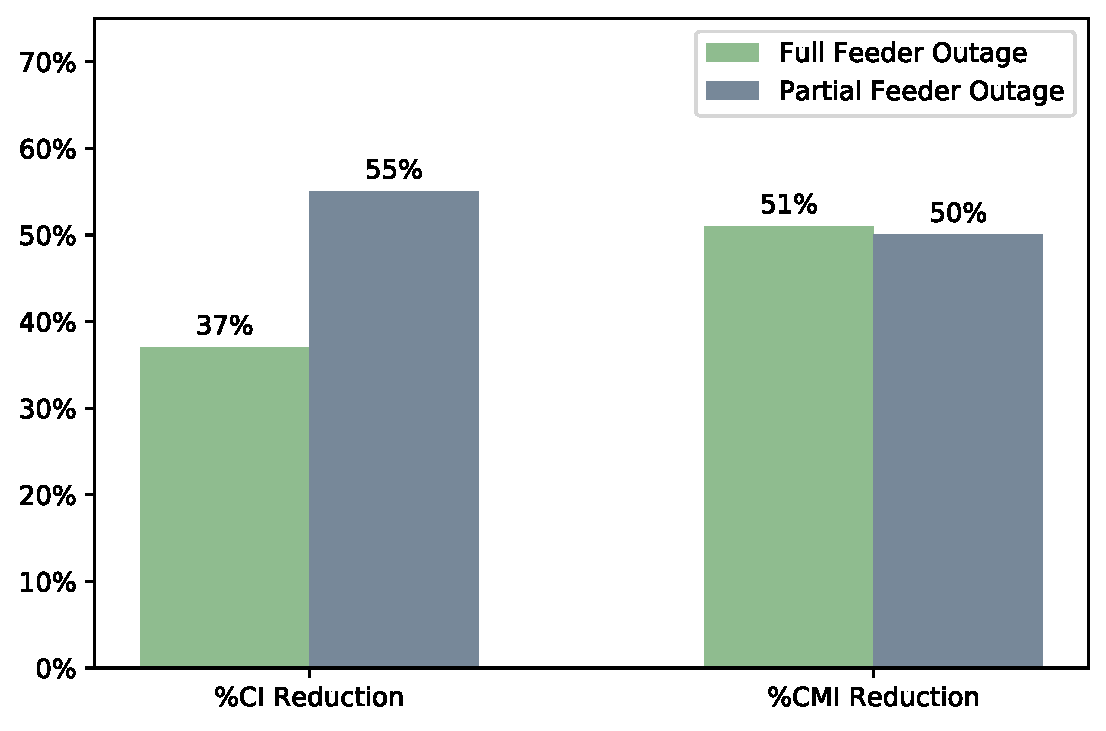
\includegraphics[scale = 0.5]{_introduction/fig/type_outage}
	\caption{FLISR effects on the number of customers interrupted (CI) and customer minutes of interruption (CMI) by the type of outage from USDON2016 \cite{USDepartmentofEnergy2016}.}
	\label{ch-introduction:fig:type_outage}
\end{figure}
\begin{figure}
    \centering
	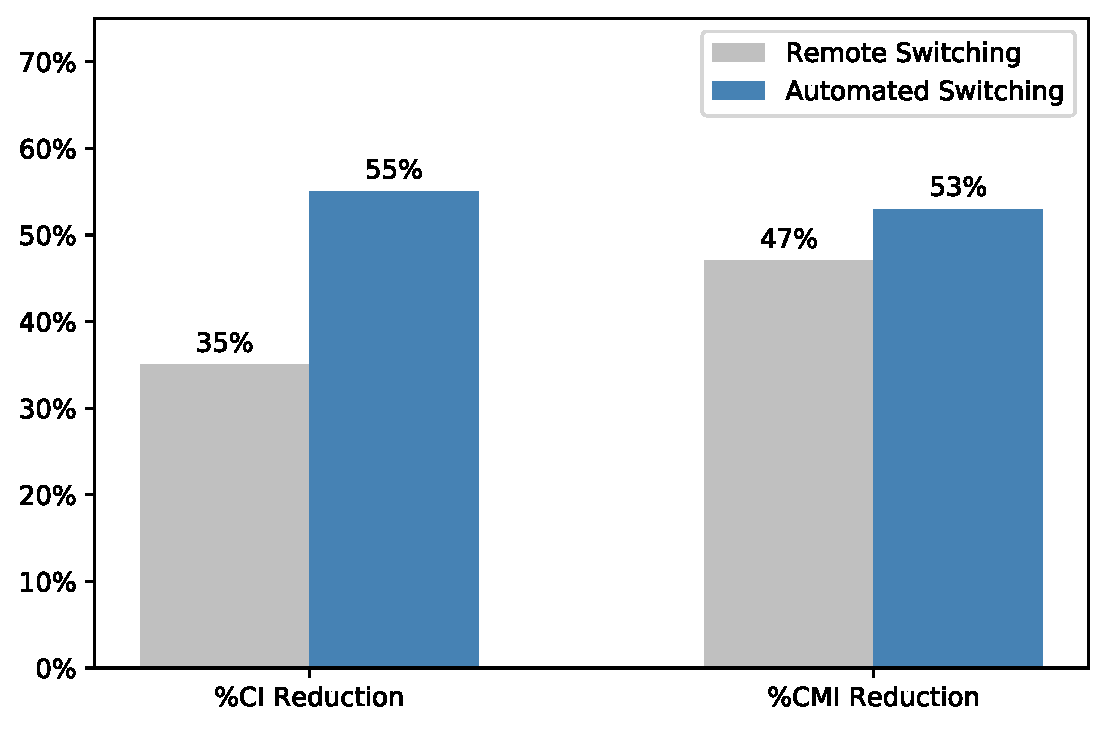
\includegraphics[scale = 0.5]{_introduction/fig/type_scheme.pdf}
	\caption{FLISR effects on the number of customers interrupted (CI) and customer minutes of interruption (CMI) by the type of FLISR operating scheme from USDON2016 \cite{USDepartmentofEnergy2016}.}
	\label{ch-introduction:fig:type_scheme}
\end{figure}

Figures \ref{ch-introduction:fig:type_outage} and \ref{ch-introduction:fig:type_scheme} show the reduction 
in CI and CMI by the type of outage and by type of FLISR scheme, respectively. The first figure states the 
number of customers interrupted decreases by 55$\%$ in a partial feeder outage, while the time of a full 
feeder outage decreases by 51$\%$. On the other hand, the second figure establishes that both CI and CMI 
have a further reduction when the FLISR scheme is automatic. Lastly, it should be pointed out these 
reductions improve directly the reliability indices mentioned before. 

As aforementioned, three stages constitute the FLISR scheme. The last stage is Service Restoration, one of the
most relevant strategies to enhance the resilience of DNs \cite{Shen2018}, and which is the main topic of this work.
%The problem is raised in the next section. 